\section{Vorlesung 18.05.2017}

\subsection{Dynamische Systeme} % FIXME

\subsubsection{Kontinuierliche dynamische Systeme}

\begin{description}
    \item[Dynamisches System] Differentialgleichung \quad $ \dot{x} = f(x) $
    \item[Fixpunkte] $ \dot{x} = 0 \quad f(\hat{x}) = 0 $
\end{description}

\paragraph{Stabilität von Fixpunkten}
\begin{itemize}
    \item durch Linearisierung $ f(x) = f(\hat{x}) + J(\hat{x}) (x - \hat{x}) + \text{Rest} $
    \item Eigenwerte $ \lambda_1 \dots \lambda_n $ \quad ($ n $ Variablen)
        \begin{itemize}
            \item $ \Re(\lambda_i) < 0 $ \quad stabile "`Richtung"'
            \item $ \Re(\lambda_i) > 0 $ \quad instabile "`Richtung"'
            \item "`Richtung"' \quad 1. reeller Eigenwert/Eigenvektor
            \item Ein Paar konjugiert-komplexer EW/EV $ \rightarrow $ Wirbel
        \end{itemize}
\end{itemize}

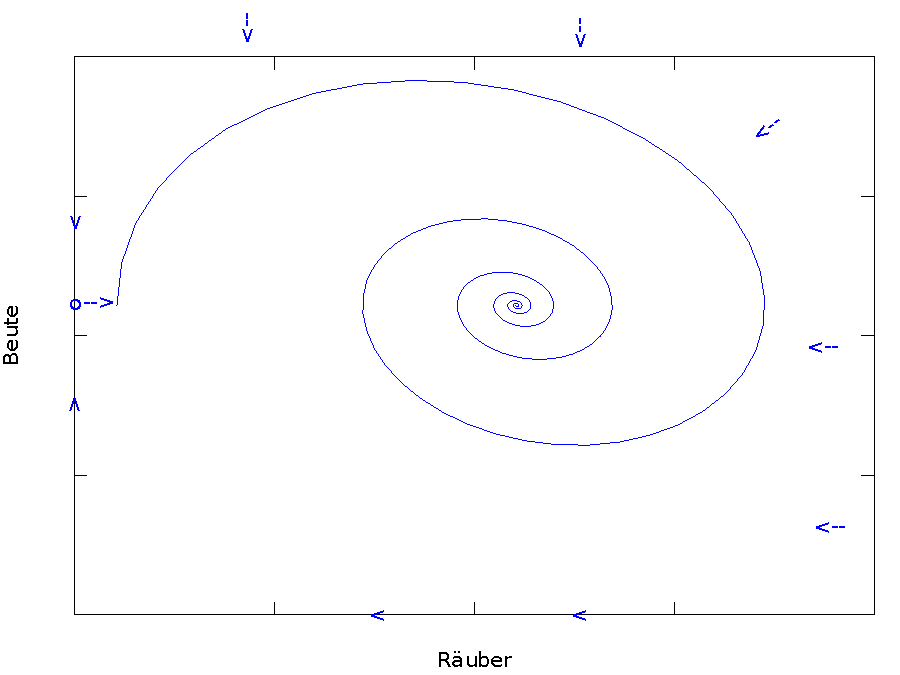
\includegraphics[width=\textwidth]{lectures/170518/pix/trajektorie_1.pdf}

\subsubsection{Diskrete dynamische Systeme}
\begin{math}
    x' = x + f(x) \\
    x' = x \; \Leftrightarrow \; f(\hat{x}) = 0 \\
    \epsilon := x - \hat{x} \\
    \epsilon' = x' - \hat{x} = \underbrace{x - \hat{x}}_{\epsilon} + \underbrace{f(\hat{x} + \epsilon)}_{f(\hat{x}) + J(\hat{x}) \cdot \epsilon = 0} \\
    \epsilon' = \epsilon + J(\hat{x}) \cdot \epsilon = [I + J(\hat{x})] \cdot \epsilon \\
    | \Re(\mu_i) | < 1 \\
    \text{Eigenwerte } \mu_i \text{ von } I + J(\hat{x}) \text{ sind } 
    1 + \lambda_i \text{, wobei } \lambda_i \text{ die Eigenwerte von } 
    J(\hat{x}) \text{ sind.} \\
    |1 + \Re(\lambda_i)| > 1 \quad \text{instabil} \\
    |1 + \Re(\lambda_i)| < 1 \quad \text{stabil} \\
    \epsilon' = \epsilon + J(\hat{x}) \cdot \epsilon = [I + J(\hat{x})]
    \cdot{\epsilon} \\
    |\Re(\mu_i)| < 1
\end{math}

\begin{description}
    \item[Heterokliner Orbit] besteht aus Sattelpunkten und deren Verbindungen
    \item[$\omega$-Limit] einer Trajektorie $ x(t, x_0) $ ist die Menge aller Punkte, deren
        $ x(t, x_0) $ unendlich oft beliebig nahe kommt
        $ y \in w(x_0) \Leftrightarrow \exists \text{ Folge } t_k, t_{k+1} \leqslant t_k + 1, 
        \text{ sodass für alle } \epsilon > 0 \text{ ein } k_{\epsilon} 
        \text{ existiert mit } | x(t_k, x_0) - y | < \epsilon $ für alle 
        $ k \geqslant k_{\epsilon} $
\end{description}

\subsection{Für dynamische Systeme in der Ebene}
Eine ODE in der Ebene mit stetig differenzierbare Vektorfeld $f$ hat nur folgende Typen von $\omega$-Limits:
\begin{itemize}
    \item Fixpunkte
    \item Zyklen (periodische Orbits)
    \item Homokline oder heterokline Orbits
\end{itemize}

DAS STIMMT FÜR DIE DISKRETEN MODELLE NICHT!

\subsection{Bifurkation}
$ \dot{x} = f(x, \underbrace{\mu}_{\mathclap{\text{Parameter}}}) $ \qquad 
alles hängt nun explizit von $  \mu $ ab \\
$ \Rightarrow $ Fixpunkte $ \hat{x}(\mu) $ \\
Stabilität der Fixpunkte $ J(\hat{x}, \mu) $ \\\\
3 Grafiken \\\\
Diagramme der Fixpunkte, Zyklen, Sattelverbindungen heißen \emph{Phasenportraits}. \\
Phasenportraits sind äquivalent, wenn sie durch stetig differenzierbare Deformationen ineinander überführbar sind ("Verzerren einer Gummifläche"). 
\begin{description}
    \item[Bifurkation:] Übergang zwischen nicht-äquivalenten Phasenportraits in Abhängigkeit von $\mu$
    \item[Einfachster Fall:] Stabilität von einem Fixpunkt ändert sich
    \item[Darstellung:] Bifurkationsdiagramme
\end{description}

Bild \\\\
Für $ \mu\*: \Re(\lambda) = 0 \quad $ für $ J(\hat{x}(\mu\*)) $
\paragraph{Saddle node bifurcation}
Anzahl der Fixpunkte ändert sich um 2
\paragraph{Pitchfork bifurcation}
Aus 1 mach' 3 \\
stabiler Fixpunkt $\rightarrow$ 1 stabiler, 2 instabile FP
\paragraph{Transkriptische Bifurkation}
2 Fixpunkte tauschen Stabilität aus
\paragraph{Hopf-Bifurkation}
\paragraph{Kein spezieller Name (teilweise "`heterokline Bifurkation"')}

\subsection{Deterministisches Chaos}
Idee: De-facto Unvorhersagbarkeit des Langzeitverhaltens
$ x_0 \cdot \rightarrow x(t, x_0) = y(t) $ \\
$ x_0' \cdot \rightarrow x(t, x_0') = y'(t) $ \\
$ | y(x) - y'(x) | > \epsilon \cdot \exp(\alpha t) \quad \text{ für } \alpha > 0 $ \\
$ | x_0 - x_0' | = \epsilon $ \\
"`driftet exponentiell auseinander"' \\
Fehler in Bestimmung der Anfangsbedingung wird exponentiell verstärkt $\rightarrow$ genaue Vorhersagen nur für kurze Zeiten möglich
\paragraph{Chaotische Attraktoren}
Mengen $A$, die anziehend, im Sinn \\
\begin{itemize}  % FIXME
    \item jede Trajektorie aus der Nähe von $A$ hat ihren $\omega$-Limes in $A$ (ATTRAKTOR)
    \item Für fast alle Ausgangsbedingungen $x_0, x_0'$ gilt die Chaos-Bedingung
    \item[2D] für brave DGL: kein Chaos
    \item[3D] Chaos existiert
\end{itemize}

\subsection{Musterbildung}
$ x(t) \rightsquigarrow u(t) \qquad \dots \qquad u(\underbrace{x}_{\text{Raum}}, \underbrace{t}_{\text{Zeit}}) $ \\
Räumlich homogen $\Leftrightarrow$ unabhängig von der Raum-Koordinate $x$ \\
$ \dot{u} := \frac{\partial u}{\partial t} = \underbrace{f}_{\mathclap{\text{Vektorfeld}}}(u) $

\subsection{Diffusion}
Teilchenstrom $J$ \\
$ \frac{\partial c}{\partial t} = \frac{\partial J}{\partial x} = -D \frac{\partial^2}{\partial x^2} c $ \qquad Kontinuitätsgleichung \\
$ J = -D \frac{\partial c}{\partial x} $ \qquad Fick'sches Gesetz \\
$ \frac{\partial u}{\partial t} = - D \frac{\partial^2}{\partial x^2} u + f(u) $ \qquad in einer R.-Dim. \\
$ \frac{\partial}{\partial t} u = -D \cdot \underbrace{\Delta}_{\mathclap{\text{Laplace-Diff.-Operator}}} u 
+ f(u) \qquad \Delta u = \sum\limits_{i=1}^{\text{Dim.}} \frac{\partial^2}{\partial x_i^2} u $

\subsubsection{Einschub: Simulation von Reaktions-Diffusionsgleichungen}
$ \frac{\partial u}{\partial t} = \frac{u(t + \delta t) - u(t)}{\delta t} $ \\

--- BILD vom Gitter ---\\
$ (\hat{x}_1 + \delta_{x_1}, \hat{x}_2) $ \\
$ \hat{x} = (\hat{x}_1, \hat{x}_2) $ \\

$ \frac{\partial u}{\partial x_1}(\tilde{x}) = \frac{u(\hat{x}_1 + \delta \overbrace{\hat{x}_1}^{\mathclap{\hat{x}_2 \text{ fix}}}) - 
u(\overbrace{\hat{x}_1}^{\mathclap{\hat{x}_2 \text{ fix}}})}{\delta x_1} $ \\
$ \frac{\partial u}{\partial x_1}(\tilde{\tilde{x}}) = \frac{u(\hat{x}_1, \hat{x}_2) - u(\hat{x}_1 - \delta \hat{x}_1, \hat{x}_2)}{\delta x_1} $ \\

$ \frac{u(\hat{x}_1 + \delta x_1, \hat{x}_2)}{\delta x_1} - \frac{u(\hat{x}_1, \hat{x}_2) - u(\hat{x}_1 - \delta x_1, \hat{x}_2)}{\delta x_1} $ \\
$ \frac{u(\hat{x}_1 + \delta x_1, \hat{x}_2) + u(\hat{x}_1 - \delta x_1, \hat{x}_2) - 2u(\hat{x}_1, \hat{x}_2)}{(\delta x_1)^2} $ \\

$ \Delta u = \frac{1}{(\delta x)^2} \quad \cdot \quad \sum\limits_{\mathclap{\text{Nachbarn } \hat{y} \text{ von }x}}(u(\hat{y}) - u(\hat{x})) $ \\
Ersetze den kontinuierlichen Raum durch ein $d$-dimensionales Gitter mit Abständen $l$ \\
$ \Delta u(x) \rightarrow \frac{1}{l^2} \cdot \overbrace{\sum\limits_{\mathclap{y \in N(x)}}(u(y, t) - u(x, t))}^{\hat{\Delta}} $ \\
$ \frac{u(t - \delta t) - u(t)}{\delta t} = -D \cdot \frac{1}{l^2} \cdot \hat{\Delta} u + f(u) $ \\
$ u(x, t + \delta t) = u(x, t) -D \frac{1}{l^2} \hat{\Delta} u(x, t) + f(u(x, t)) $ \\
